%                                                                 
% AA vers. 9.1, LaTeX class for Astronomy & Astrophysics - modified to 9.2
%
%                                                       (c) EDP Sciences
%-----------------------------------------------------------------------
%
%\documentclass[referee]{aa} % for a referee version
%\documentclass[onecolumn]{aa} % for a paper on 1 column  
%\documentclass[longauth]{aa} % for the long lists of affiliations 
%\documentclass[letter]{aa} % for the letters 
%\documentclass[bibyear]{aa} % if the references are not structured 
%                              according to the author-year natbib style

%
\documentclass[a4paper]{aa} % a&a template, on a4 because we're european thank you very much

\usepackage{natbib, twoopt} % a&a uses this
\bibpunct{(}{)}{;}{a}{}{,} % to follow the A&A style
%
\usepackage{amsmath, mathtools} % standard for math
%\usepackage{mathptmx} % change math font (?, might be doing nothing)
\usepackage{siunitx} % SI units support
\usepackage{graphicx} % make figures
\usepackage{subcaption} % make subfigures
\usepackage{lipsum} % lorem ipsum, a&a examples were using this
\usepackage{url} % make url links
\usepackage[hyphenbreaks]{breakurl} % allow breaking urls
\usepackage{xcolor} % make colour names available (used for links)
\definecolor{cobalt}{rgb}{0.06, 0.2, 0.65} % new color
% a&a example stuff
\usepackage{lscape}             % to rotate a single page table, example in appendix.
                                % For landscape tables, see the longtable examples.
\usepackage{placeins}           % useful with \FloatBarrier, to keep 
                                % onecolumn floats from drifting to the next section
%%%%%%%%%%%%%%%%%%%%%%%%%%%%%%%%%%%%%%%%
%\usepackage{txfonts}
\usepackage[varg]{txfonts} % change general font as a&a recommends
%%%%%%%%%%%%%%%%%%%%%%%%%%%%%%%%%%%%%%%%
\usepackage[colorlinks, breaklinks]{hyperref} % linking inside pdf, with custom colours and allow wrapping links
% orange numbers for sections etc, citations in red, urls in blue
\hypersetup{%
  colorlinks = true,
  linkcolor  = orange,
  citecolor = red,
  urlcolor = blue,
  pdftitle={Cosmology II Project}
}
% To add links in your PDF file, use the package "hyperref"
% with options according to your LaTeX or PDFLaTeX drivers.
%

% remove warnings about empty links when using hyperref
% https://tex.stackexchange.com/questions/345764/journal-class-shows-package-hyperref-warning-suppressing-link-with-empty-targe
% and add hyperlinks to citations
% https://github.com/yangcht/AA-bibstyle-with-hyperlink
\makeatletter
% fix the page number
\renewcommand*\aa@pageof{, page \thepage{} of \pageref*{LastPage}}
% change some other displayed information, this is not a formal A&A paper after all
\renewcommand*\aa@numarticle{Cosmology II numerical project} % changing article "number" since this isn't published, don't mind the hack
% display in top box at the beginning
\renewcommand*\aa@manuscriptname{%
  templated numerical project
  \hspace{\stretch{1}}%
  \copyright UiO \the\year
}
% top text on even pages
\renewcommand*\aa@textidlineempty{{\slshape A\&A template:}\ Cosmology II}

% required for the hyperlinks, see https://github.com/yangcht/AA-bibstyle-with-hyperlink
\newcommandtwoopt{\citeads}[3][][]{\href{http://adsabs.harvard.edu/abs/#3}%
    {\def\hyper@linkstart##1##2{}%
     \let\hyper@linkend\@empty\citealp[#1][#2]{#3}}}
\newcommandtwoopt{\citepads}[3][][]{\href{http://adsabs.harvard.edu/abs/#3}%
    {\def\hyper@linkstart##1##2{}%
     \let\hyper@linkend\@empty\citep[#1][#2]{#3}}}
\newcommandtwoopt{\citetads}[3][][]{\href{http://adsabs.harvard.edu/abs/#3}%
    {\def\hyper@linkstart##1##2{}%
     \let\hyper@linkend\@empty\citet[#1][#2]{#3}}}
\newcommandtwoopt{\citeyearads}[3][][]%
    {\href{http://adsabs.harvard.edu/abs/#3}
    {\def\hyper@linkstart##1##2{}%
     \let\hyper@linkend\@empty\citeyear[#1][#2]{#3}}}

% custom hack to make eprint command have an actual arxiv link
\renewcommand*\eprint[2][]{%
{\tt\if!#1!#2\else{\href{https://arxiv.org/abs/#2}{\ignorespaces#1\arxivprefixesep\ignorespaces#2}}\fi}%
}
\makeatother


\begin{document} 


   \title{Make a suitable title: my paper on the cosmic microwave background and formation of structures in our Universe}
   \titlerunning{Cosmology II Project}

   \subtitle{AST5220: Cosmology II}

   \author{Candidate 15003
          %\inst{1}
          }

   \institute{Institute of Theoretical Astrophysics,  
   University of Oslo,  0315 Oslo,  Norway\\
             }

   \date{Received \today}
   %\date{Received September 15, 1996; accepted March 16, 1997}

%-------------------------------------------------------------------
%-------------------------------------------------------------------
% \abstract{}{}{}{}{} 
% 5 {} token are mandatory
 
  \abstract
  % context heading (optional)
  % {} leave it empty if necessary  
   {Something about a CAMB solver}
  % aims heading (mandatory)
   {Cosmological simulations}
  % methods heading (mandatory)
   {Calculations are done}
  % results heading (mandatory)
   {Results are resulted}
  % conclusions heading (optional), leave it empty if necessary 
   {An abstract for the paper. Describe the paper. What is the paper about, what are the main results, etc.}

   \keywords{cosmic microwave background --
                large-scale structure of Universe --
                %structure formation --
                recombination
               }

   \maketitle
%
%-------------------------------------------------------------------

%-------------------------------------------------------------------
\section{Introduction}

Write an introduction here. 
Give context to the paper. 
Citations to relevant papers. 
You only need to do this in the end for the last milestone.
   
%-------------------------------------------------------------------

%\FloatBarrier
\section{Milestone I}\label{sec:milestone_1}
In this milestone, we establish the so-called background cosmology of our universe for the simulation. We focus on some rough supernova fitting to give an initial target for the spacetime metric and relative energy densities we will work with.

Citations: \citet{baumannLectureNotesCosmology2017}, \citet{dodelsonModernCosmology2003} and \citep{callinHowCalculateCMB2006, wintherCosmologyIILecture2024, huCompleteTreatmentCMB1998}

\subsection{Theory}
The scale factor $a$ is used as the main time-ish variable - $a$ is not a time but since time, size of the universe, and cosmic distances are all closely related it can fulfill the role of a time variable nonetheless, and describe the evolution of our simulated universe \citep{wintherCosmologyIILecture2024}. The scale factor is a dimensionless quantity.

For numerical work we use the variable $x \equiv \log a$, this is for numerical stability over large timescales with highly variable quantities. 

We also consider the cosmic time $t$, and in theory $a$ is dependent on $t$, $a(t)$, but in practice we derive the cosmic time $t$ from $x$ (and thus $a$) and not the other way around, see eq. \ref{eq:t_of_x}.

We define $a_0$ as the value of the scale factor today, such that $a_0 \equiv a(t_{\text{today}}) \equiv 1$. Note that $x_0 = 0$. In general, subscript $_0$ indicates the value of a parameter as measured in the current day.

Another related quantity is the redshift $z$, this is also $z_0 = 0$ in the present day. As observers we must by definition be at zero redshift, after all. Redshift is given by $1+z = a_0 / a(t) = 1/a$.

\newpage
Fiducial cosmology and initial parameter values taken from the Planck 2018 results \citep{collaborationPlanck2018Results2020}. Input parameters are listed at \ref{eq:input_params}.

\begin{equation}\label{eq:input_params}
\begin{aligned}
h &= 0.67, \\
T_{\rm CMB 0} &= 2.7255\,\unit{K}, \\
N_{\rm eff} &= 3.046, \\
\Omega_{\rm b 0} &= 0.05, \\
\Omega_{\rm CDM 0} &= 0.267,\\
\Omega_{k 0} &= 0, \\
\Omega_{\nu 0} &= N_{\rm eff}\cdot \frac{7}{8}\left(\frac{4}{11}\right)^{4/3}\Omega_{\gamma 0}, \\
\Omega_{\Lambda 0} &= 1 - (\Omega_{k 0}+\Omega_{b 0}+\Omega_{\rm CDM 0}+\Omega_{\gamma 0}+\Omega_{\nu 0}),\\
n_s &= 0.965, \\
A_s &= 2.1\cdot 10^{-9}, \\
Y_p &= 0.245, \\
z_{\rm reion} &= 8, \\
\Delta z_{\rm reion} &= 0.5, \\
z_{\rm He-reion} &= 3.5, \\
\Delta z_{\rm He-reion} &= 0.5.
\end{aligned}
\end{equation}

\subsubsection{Friedmann equation}
Rather than dealing with the full Einstein equations directly, it is possible to derive the Friedmann equation in order to describe the expansion of the universe, this is eq. \ref{eq:Friedmann} \citep{wintherCosmologyIILecture2024}.

\begin{equation}\label{eq:Friedmann}
\boxed{H = H_0 \sqrt{ \Omega_{M 0} a^{-3} + \Omega_{R 0} a^{-4} + \Omega_{k 0} a^{-2} + \Omega_{\Lambda 0}}}\,,
\end{equation}

where the $\Omega_{X}$ are density parameters describing relative density of their respective form of energy contributing to the expansion of the universe. Density parameters are dimensionless. Subscript $_0$ indicates a value for the universe of today, since we as observers are by definition at $x=z=0$.

$\Omega_{M} = (\Omega_{b}+\Omega_{\rm CDM})$ is a composite density parameter describing non-relativistic matter (baryons and cold dark matter), and $\Omega_{R} = (\Omega_{\gamma} + \Omega_{\nu})$ is a composite density term for radiation (photons and neutrinos).
$\Omega_{\Lambda}$ is the density parameter for dark energy.
$\Omega_{k}$ is a curvature term, and not properly an energy density. However, it contributes to the Friedmann equation as if it were a normal matter fluid with equation of state $\omega = -1/3$. This term prescribes negative curvature when $<0$, positive curvature when $>0$, and a spatially flat universe when $=0$. Our universe is observationally confirmed to be very close to flat \citep{bennettNineYearWilkinsonMicrowave2013}, so this term should be close to $0$. 

The unit of $H$ is slightly ambiguous, as in SI units both \unit{(km \per s)\per Mpc} and the simplified \unit{1 \per s} are used. The first way of writing the unit is more intuitive, as it relates to the change in velocity of distant galaxies based on their distance from the observer (us), aka Hubble's law. \unit{1 \per s} is technically correct but interpreting the Hubble parameter as a frequency is not helpful. For the Friedmann equation and derived quantities, we mostly skip this problem by keeping $H$ in "units of $H$", using the value of the Hubble parameter today ($H_0$) as a constant which gives the right units to any $H$ that pops up.

For numerical work, we calculate the constant $H_0$ by adding the right units to a dimensionless constant $h$ (eq. \ref{eq:little_h}), which is commonly used and reported in the literature \citep{crotonDamnYouLittle2013}. $h$ is one of the input observables for our numerical simulation, so we use the $0.67$ value reported by Planck 2018 \citep{collaborationPlanck2018Results2020}.

\begin{equation}\label{eq:little_h}
H_0 = 100 * h \enspace \unit{km.s^{-1}.Mpc^{-1}}
\end{equation}

\subsubsection{More stuff}

Paper with supernova fitting data \citet{betouleImprovedCosmologicalConstraints2014}.

Equation for critical density of the universe today \ref{eq:critical_density}

\begin{equation}\label{eq:critical_density}
\rho_{c0} \equiv \frac{3H_0^2}{8\pi G} \enspace \unit{kg.m^{-3}}
\end{equation}

\begin{equation}\label{eq:t_of_x}
t(x) = \int_0^a \frac{da}{aH} = \int_{-\infty}^x \frac{dx}{H(x)} \quad [\text{unit \unit{s}, can convert to \unit{\giga yr} etc.}]
\end{equation}

\subsection{Implementation details}
We run a Markov chain Monte Carlo simulation on a large number of parameter combinations, in order to test numerical fitting to real supernova data. This ensures our background parameters and simulation is sensible, before we add perturbations to simulate a dynamic universe development through time.

\subsection{Results}
See figs. \ref{fig:milestone_1_cosmic_vs_conformal_time}, \ref{fig:milestone_1_luminosity_distance}, \ref{fig:milestone_1_etaHp_over_c_of_x}, \ref{fig:milestone_1_Omega_i_of_x}, \ref{fig:milestone_1_supernovafitting_confidence_regions}. Overall these figures seem ok, except that the supernova fitting in fig. \ref{fig:milestone_1_luminosity_distance} misses systematically, especially at the beginning. There is probably some bug involved, since the shape seems correct.

Best-fit parameters are
Best h: 0.706857,
Best H0: 70.6857 km/s/Mpc,
Best OmegaM: 0.268287,
Best OmegaK: 1.84807e-05,
Best OmegaLambda: 0.731694519

Via the cosmic time, the calculated current age of the Universe is: $13.849 * 10^9$ yrs.
This is pretty close to 13.79 billion years, the current accepted estimate.

\begin{figure}[h!tbp]
\centering
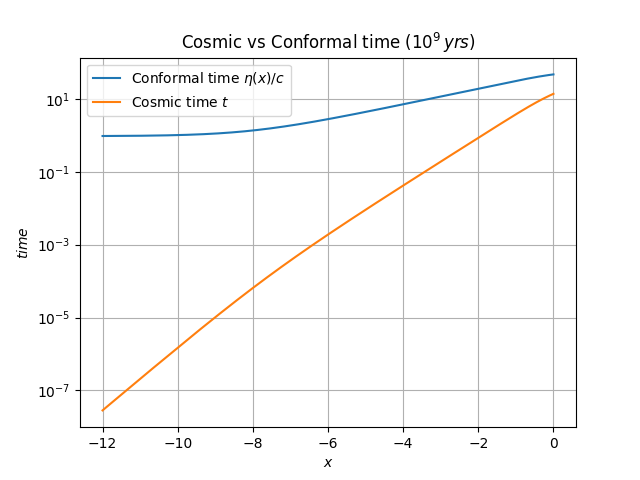
\includegraphics[width=0.4\textwidth]{../Milestone 1/Plots/cosmic_vs_conformal_time.png}
\caption{Cosmic and conformal time plotted against the expansion of the universe. The cosmic time evolves almost linearly, as we'd expect.}
\label{fig:milestone_1_cosmic_vs_conformal_time}
\end{figure}

\begin{figure}[h!tbp]
\centering
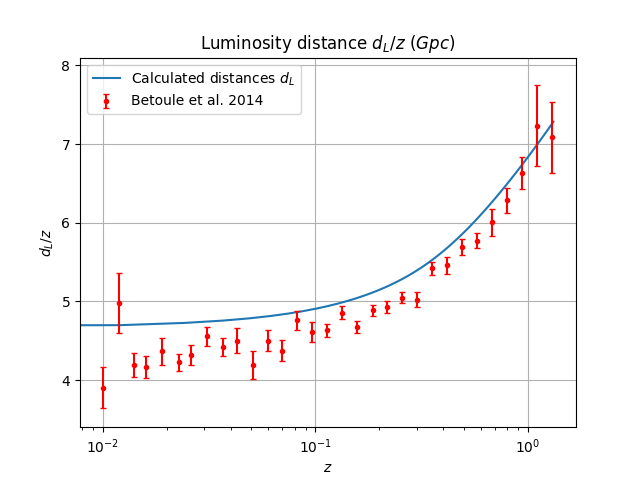
\includegraphics[width=0.4\textwidth]{../Milestone 1/Plots/luminosity_distance.png}
\caption{Luminosity distance against redshift, with larger redshifts representing objects further away. This evolution is strongly related to the Hubble parameter and Hubble's law.}
\label{fig:milestone_1_luminosity_distance}
\end{figure}

\begin{figure}[h!tbp]
\centering
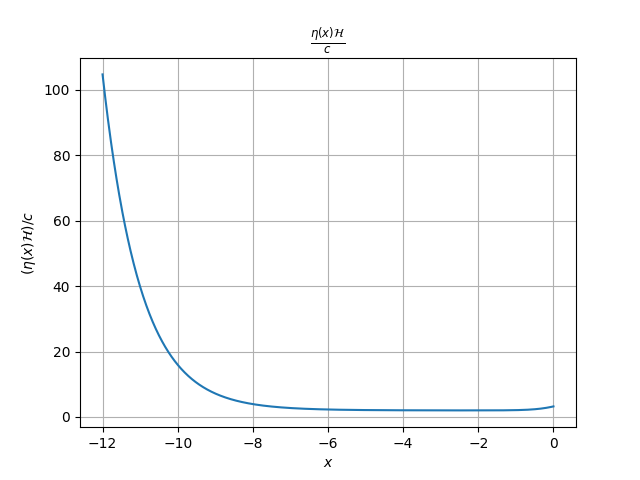
\includegraphics[width=0.4\textwidth]{../Milestone 1/Plots/etaHp_over_c_of_x.png}
\caption{A plot of the conformal Hubble factor $\mathcal{H} = aH$, scaled against the analytical solution of the Friedmann equation in the radiation dominated era ($\eta \simeq \frac{c}{\mathcal{H}}$). This should converge to $1$ the more radiation dominated the universe is, and shows the correct exponential decay compared to the decay of relativistic matter seen in fig. \ref{fig:milestone_1_Omega_i_of_x}, if not the right value at the beginning of the plot.}
\label{fig:milestone_1_etaHp_over_c_of_x}
\end{figure}

\begin{figure}[h!tbp]
\centering
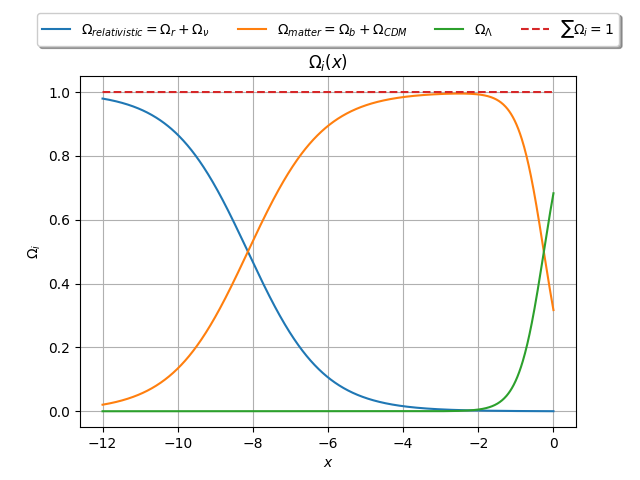
\includegraphics[width=0.4\textwidth]{../Milestone 1/Plots/Omega_i_of_x.png}
\caption{The evolution of the various energy components from the Friedmann equation. We clearly see the three eras of radiation-domination, matter-domination, and dark energy beginning to dominate right around the present day, as expected. For reference, the sum of the components is calculated at every point and plotted at the top - this exeeding 100\% energy at any point would be very problematic, but it stays perfectly at 1.}
\label{fig:milestone_1_Omega_i_of_x}
\end{figure}

\begin{figure}[h!tbp]
\centering
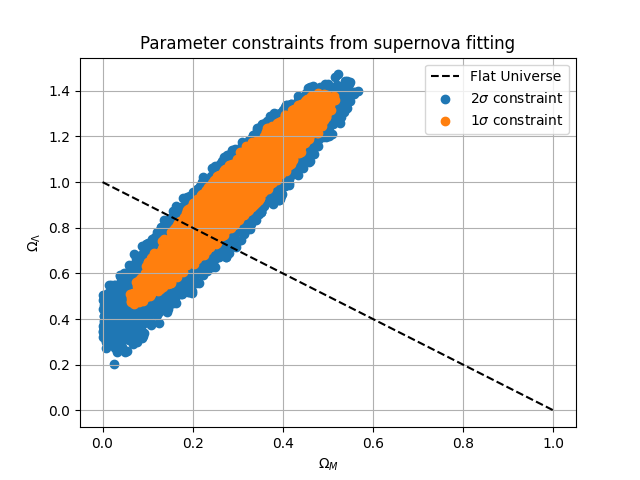
\includegraphics[width=0.4\textwidth]{../Milestone 1/Plots/supernovafitting_confidence_regions.png}
\caption{A scatter plot of the various parameter combinations that were attempted for fitting by the MCMC. Parameters outside the blue area are extremely unlikely. For reference, the combinations corresponding to a spatially flat universe are the ones on the dotted black line. Since we know observationally that our universe is close to flat, a dark energy content of about 60-80\% is likely, with a corresponding matter density of about 20-40\%.}
\label{fig:milestone_1_supernovafitting_confidence_regions}
\end{figure}

\section{Milestone II}\label{sec:milestone_2}
With fundamental cosmology established in sec. \ref{sec:milestone_1}, we can now describe the baseline or so-called "background" behaviour of our Universe, with a relatively simple evolution of cosmological paremeters as the universe expands (refer fig. \ref{fig:milestone_1_Omega_i_of_x}). Now we wish to look backwards from our current time, and compute the path of photons travelling towards a current-day observer from the early universe.

In order to study the behaviour of photons and thermal evolution of the early universe, we consider it to be a large continuous fluid, specifically a hot plasma. The thermodynamics and statistical mechanics for this are described in \citet[][chap.~x]{baumannLectureNotesCosmology2017} and \citet[][chap.~x]{dodelsonModernCosmology2003}, while the specific Boltzmann formalism utilized is that of \citet[][]{wintherCosmologyIILecture2024}, \href{https://cmb.wintherscoming.no/theory_thermodynamics.php#thermo}{which can be found here}.

\subsection{Theory}
The theory behind this milestone.

Start with eqs. \ref{eq:tau_integral} and \ref{eq:tau_ODE}.

\begin{equation}\label{eq:tau_integral}
\tau(\eta) = \int_{\eta}^{\eta_0} n_e \sigma_T a d\eta'
\end{equation}

\begin{equation}\label{eq:tau_ODE}
\boxed{\tau' = \frac{d\tau}{dx} = -\frac{c n_e \sigma_T }{H}.}
\end{equation}

We wish to compute the fractional electron density given by \ref{eq:fractional_electron_density}, where we assume all baryons are protons and there are no heavier elements. This approximation is acceptable for getting a simple reionization with clear falloff of electrons as they get absorbed into hydrogen atoms. By including ionization into Helium, our resulting ionization plot would have multiple bumps for ionization into different states of Hydrogen+Helium.


\begin{equation}\label{eq:fractional_electron_density}
\boxed{X_e \equiv n_e / n_H}, \text{ with } \,\, n_H = n_b \approx \frac{\rho_b}{m_H} = \frac{\Omega_{b0} \rho_{c0}}{m_H a^3}
\end{equation}


Saha approximation \ref{eq:saha_approx}

\begin{equation}\label{eq:saha_approx}
\boxed{\frac{X_e^2}{1-X_e} = \frac{1}{n_b} \left(\frac{m_e
T_b}{2\pi}\right)^{3/2} e^{-\epsilon_0/T_b}}
\end{equation}

Peebles equation \ref{eq:peebles_equation}, with the supporting definitions in eq. \ref{eq:peebles_quantities_definition}.

\begin{equation}\label{eq:peebles_equation}
\boxed{\frac{dX_e}{dx} = \frac{C_r(T_b)}{H} \left[\beta(T_b)(1-X_e) - n_H
\alpha^{(2)}(T_b)X_e^2\right],}
\end{equation}

\subsection{Implementation details}
Something about the numerical work.

\subsection{Results}
Show and discuss the results.

%\section{Milestone III}
Some introduction about what it is all about.

\subsection{Theory}
The theory behind this milestone.

\subsection{Implementation details}
Something about the numerical work.

\subsection{Results}
Show and discuss the results.

%\section{Milestone IV}
I got completely stuck on milestone III. I was looking forward to III and finally getting to some of the physics there, too

Citations: \citet{fixsenCosmicMicrowaveBackground1996}

\subsection{Theory}
CMB and matter power spectrums, how they work and the different regimes in them. How a sum of coefficients describes the different scale components of a sky-map. Line of sight integration to calculate all the various $\Theta_\ell$-s.

How the different regimes in the power spectrum plots are affected by different shifts in cosmological parameters. Cosmic variance in the beginning at low $\ell$-s. $A_s$ for overall amplitude of the whole spectrum, $n_s$ describes tilt. The fluctuation peaks after the main peak tell us about baryon and dark matter density. Also affected by polarization, neturinos, and reionization which is why the simpler power spectrum we would have derived would be off from the Planck spectrum in this regime, while the lower $\ell$-s match fine.

The matter power spectrum tells us about the total matter component in the universe, but the interesting part is the second small peak and subsequent dampened fluctuations that tell us about the ratio of baryons to dark matter, due to the effect of baryon dragging.

The source function:

\begin{equation}\label{eq:source_function}
\begin{aligned}
    \tilde{S}(k,x) = \tilde{g}\left[ \Theta_0 + \Psi + \frac{1}{4}\Pi\right] + e^{-\tau} \left[\Psi^\prime-\Phi^\prime\right] - \\
    - \frac{1}{ck}\frac{d}{dx}(\mathcal{H}\tilde{g}v_b) + \frac{3}{4c^2k^2} \frac{d}{dx} \left[\mathcal{H}\frac{d}{dx} (\mathcal{H}\tilde{g}\Pi)\right].
\end{aligned}
\end{equation}

This describes various effects in the universe that have affected photons travelling from the surface of last scattering (the CMB photons) to us, today. The baseline movement is in the first term (hence the dependency on visibility function). The term with $\psi$ dependence is a correction due to the Sachs-Wolfe effect, the term with $\Pi$ is a correction for the effect of the photon quadropole and some polarization. The next main term is a correction for the integrated Sachs-Wolfe effect (ISW), which should have one of those neat diagrams to show how photons gain energy due to gravitational wells decaying while they are climbing out. Next up is a correction for Doppler shift, and finally a correction for angular dependence in Thompson scattering.

\subsection{Implementation details, results}
It did not work

\section{Conclusions}

   \begin{enumerate}
      \item The conditions for the stability of static, radiative
         layers in gas spheres, as described by Baker's (\citeyear{baker})
         standard one-zone model, can be expressed as stability
         equations of state. These stability equations of state depend
         only on the local thermodynamic state of the layer.
      \item If the constitutive relations -- equations of state and
         Rosseland mean opacities -- are specified, the stability
         equations of state can be evaluated without specifying
         properties of the layer.
      \item For solar composition gas the $\kappa$-mechanism is
         working in the regions of the ice and dust features
         in the opacities, the $\mathrm{H}_2$ dissociation and the
         combined H, first He ionization zone, as
         indicated by vibrational instability. These regions
         of instability are much larger in extent and degree of
         instability than the second He ionization zone
         that drives the Cephe{\"\i}d pulsations.
   \end{enumerate}

\begin{acknowledgements}
      Part of this work was supported by the German
      \emph{Deut\-sche For\-schungs\-ge\-mein\-schaft, DFG\/} project
      number Ts~17/2--1.
\end{acknowledgements}
%-------------------------------------------------------------------


%-------------------------------------------------------------------
% - use BibTeX with the regular commands:
%   \bibliographystyle{aa} % style aa.bst
%   \bibliography{Yourfile} % your references Yourfile.bib
%
% - join the .bib files when you upload your source files

\bibliographystyle{bibtex/aa_url}
\bibliography{bibtex/bibliography.bib}

%-------------------------------------------------------------------

\begin{appendix}

\FloatBarrier
\section{Code repository}
All code used for this project is available at \href{https://github.com/ericludvigs/AST5220_Cosmology_Project}{this Github repository}.
Description of code folders and places to look here.

\FloatBarrier
\section{Milestone I, extra plots}\label{app:milestone_1_extra_plots}

Evolution of some physical quantities in figs. \ref{fig:milestone_1_H_prime_of_x} and \ref{fig:milestone_1_eta_of_x}.

\begin{figure}[h!tb]
\centering
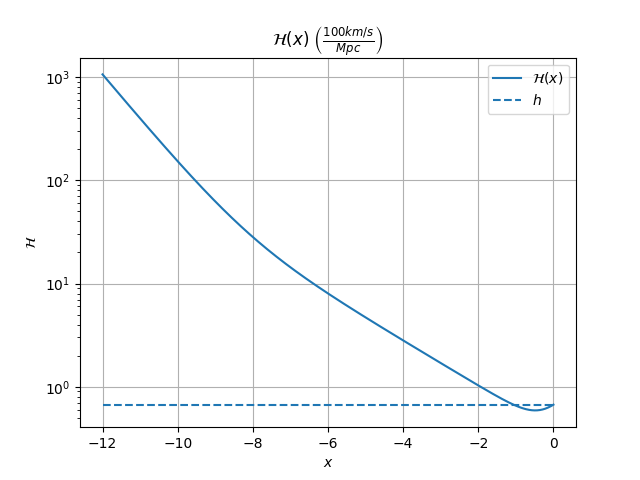
\includegraphics[width=0.4\textwidth]{../Milestone 1/Plots/H_prime_of_x.png}
\caption{Caption}
\label{fig:milestone_1_H_prime_of_x}
\end{figure}

\begin{figure}[h!bt]
\centering
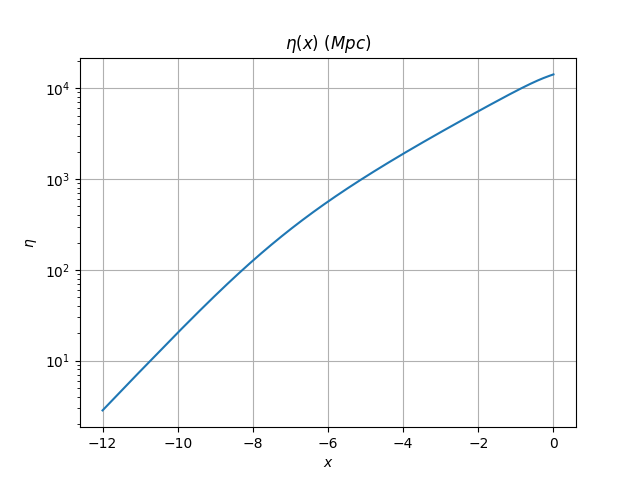
\includegraphics[width=0.4\textwidth]{../Milestone 1/Plots/eta_of_x.png}
\caption{Caption}
\label{fig:milestone_1_eta_of_x}
\end{figure}

Histograms of parameter distribution in fig. \ref{fig:milestone_1_appendix_histograms}.

\begin{figure*}[h!tb]
\centering
    \begin{subfigure}[t!]{0.4\textwidth}
    \centering
    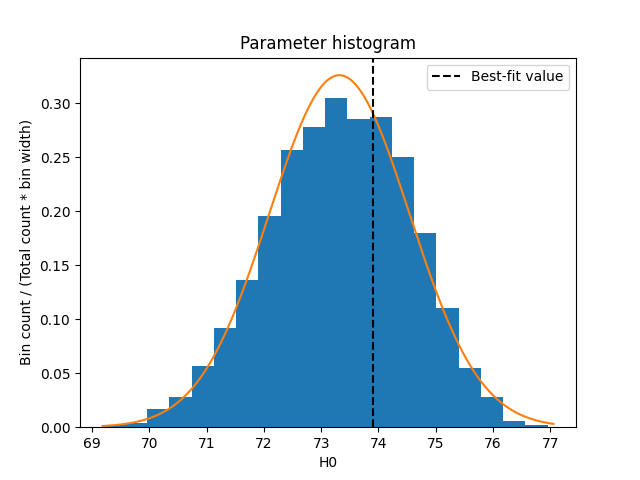
\includegraphics[width=1.0\textwidth]{../Milestone 1/Plots/H0_histogram.png}
    \caption{Caption 1}
    \label{fig:milestone_1_H0_histogram}
    \end{subfigure}
    %\hfill
    \begin{subfigure}[t!]{0.4\textwidth}
    \centering
    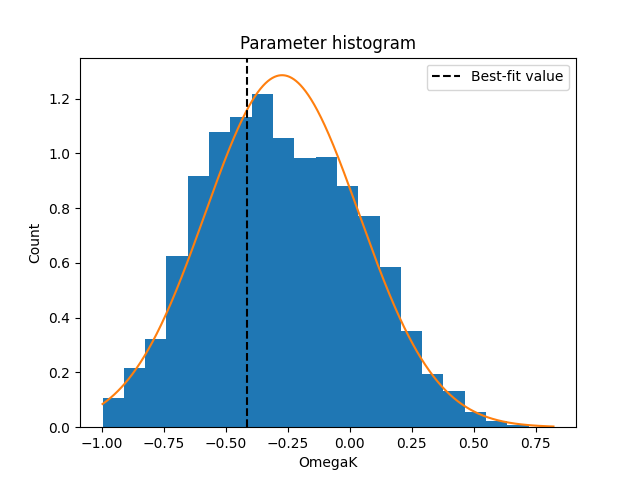
\includegraphics[width=1.0\textwidth]{../Milestone 1/Plots/OmegaK_histogram.png}
    \caption{Caption 2}
    \label{fig:milestone_1_OmegaK_histogram}
    \end{subfigure}
    \hfill
    %\hfill
    \begin{subfigure}[b!]{0.4\textwidth}
    \centering
    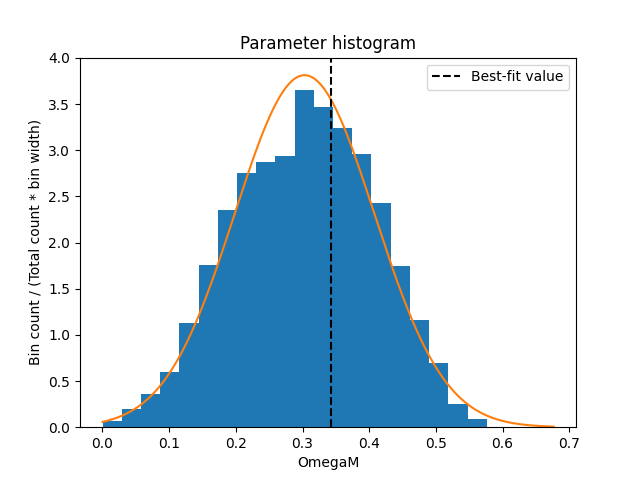
\includegraphics[width=1.0\textwidth]{../Milestone 1/Plots/OmegaM_histogram.png}
    \caption{Caption 3}
    \label{fig:milestone_1_OmegaM_histogram}
    \end{subfigure}
    \begin{subfigure}[b!]{0.4\textwidth}
    \centering
    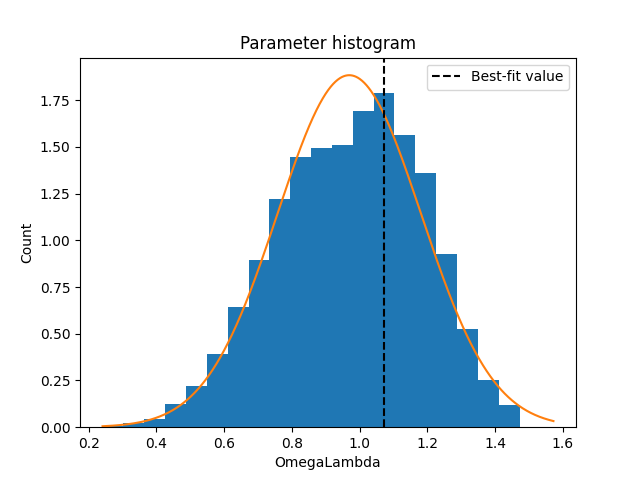
\includegraphics[width=1.0\textwidth]{../Milestone 1/Plots/OmegaLambda_histogram.png}
    \caption{Caption 4}
    \label{fig:milestone_1_OmegaLambda_histogram}
    \end{subfigure}
\caption{Whole figure caption}
\label{fig:milestone_1_appendix_histograms}
\end{figure*}

\FloatBarrier
\section{Milestone II, extra math}


\boxed{
\begin{aligned}\label{eq:peebles_quantities_definition}
C_r(T_b) &= \frac{\Lambda_{2s\rightarrow1s} + \Lambda_{\alpha}}{\Lambda_{2s\rightarrow1s} + \Lambda_{\alpha} + \beta^{(2)}(T_b)}, \,\,{\rm (dimensionless)}\\
H &,  \,\,{\rm (dimension~1/s)}\\
\Lambda_{2s\rightarrow1s} &= 8.227 \textrm{s}^{-1}, \,\,{\rm (dimension~1/s)}\\
\Lambda_{\alpha} &= H\frac{(3\epsilon_0)^3}{(8\pi)^2 n_{1s}}, \,\,{\rm (dimension~1/s)}\\
n_{1s} &= (1-X_e)n_H, \,\,{\rm (dimension~1/m^3)}\\
n_H &= (1-Y_p)\frac{3H_0^2\Omega_{b0}}{8\pi G m_H a^3}, \,\,{\rm (dimension~1/m^3)}\\
\beta^{(2)}(T_b) &= \beta(T_b) e^{3\epsilon_0/4T_b}, \,\,{\rm (dimension~1/s)}\\
\beta(T_b) &= \alpha^{(2)}(T_b) \left(\frac{m_eT_b}{2\pi}\right)^{3/2} e^{-\epsilon_0/T_b}, \,\,{\rm (dimension~1/s)} \\
\alpha^{(2)}(T_b) &= \frac{64\pi}{\sqrt{27\pi}}\frac{\alpha^2}{m_e^2}\sqrt{\frac{\epsilon_0}{T_b}}\phi_2(T_b), \,\,{\rm (dimension~m^3/s)}\\
\phi_2(T_b) &= 0.448\ln(\epsilon_0/T_b), \,\,{\rm (dimensionless)}\\
\alpha &\simeq \frac{1}{137.0359992}, \,\,{\rm (dimensionless)}
\end{aligned}
}

\end{appendix}


%-------------------------------------------------------------------
\end{document}
